\section{Appendix}\label{appendix}
We now provide the deferred proof of Theorem~\ref{AleUpper} in the following Section \S\ref{proofAleUpper} and the extension of our strategies to $n$-tadpole graphs in the subsequent Section \S\ref{ntadpoles}.
For this proof, we consider $e_{max} = (v_s, v_\ell)$, as shown in Figure \ref{Example2}.
\begin{figure}[H]
    \begin{center}
        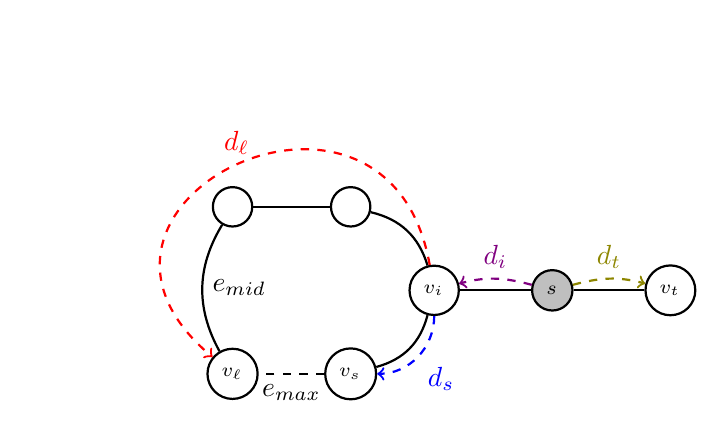
\begin{tikzpicture}[node distance={15mm}, thick, main/.style = {draw, circle}, scale=0.5] 
            \node[main, minimum size=0.5cm] (2) {$_{v_s}$ }; 
            \node[main, minimum size=0.5cm] (3) [above right of = 2] {$_{v_i}$ }; 
            \node[main, minimum size=0.5cm] (4) [above left of = 3] {};
            \node[main, fill=gray!50, minimum size=0.5cm] (6) [right of = 3] {$_{s}$ };
            \node[main, minimum size=0.5cm] (7) [left of = 2] {$_{v_\ell}$ };
            \node[main, minimum size=0.5cm] (8) [left of = 4] {};
            \node[main, minimum size=0.5cm] (9) [right of = 6] {$_{v_t}$ };
            \draw (7) [bend left] to node[right] {$e_{mid}$} (8);
            \draw (2) [bend right] to node[right] {} (3);
            \draw (3) [bend right] to node[above right] {} (4);
            \draw (3) [] to node[above] {} (6);
            \draw (2) [dashed] to node[below] {$e_{max}$} (7);
            \draw (4) [] to node[above] {} (8);
            \path [red, thick, dashed, ->] (3) edge[looseness=2.6, bend angle=90, out=100,in=140] node[above] {{$d_\ell$}} (7);
            \path [blue, thick, dashed, ->] (3) edge[out=270,in=0] node[below right] {{$d_s$}} (2);
            \path [olive, thick, dashed, ->] (6) edge[out=15,in=165] node[above] {{$d_t$}} (9);
            \path [violet, thick, dashed, ->] (6) edge[out=165,in=15] node[above] {{$d_i$}} (3);
            \draw (6) [] to node[above] {} (9);
        \end{tikzpicture} 
    \end{center}
    \caption[Tadpole example]{Tadpole Graph Example. The paths $p_\ell, p_s, p_i, p_t$ and the edges $e_{mid}$ and $e_{max}$ are marked.}
    \label{Example2}
\end{figure}

\subsection{Proof of Thm.~\ref{AleUpper}}\label{proofAleUpper}
\begin{proof} Consider the possible starting positions of the agents in a tadpole graph. We show that for any starting position a team of three agents will
    reach a competitive ratio of at most $3$, while a team of four agents reaches a competitive ratio of $2$.

\paragraph*{Starting at the end of the tail}
In this case two agents suffice to reach a competitive ratio of $1.5$. We consider $\opt_C$ to be the time needed for the exploration of the cycle by an optimal strategy.
We already know that the \textit{ALE} strategy needs at most time $1.5\opt_C$ for the exploration of a cycle. Since the exploration starts on $v_t$, an online strategy can send both agents
to $v_i$, let them explore the cycle using the \textit{ALE} strategy, and have them return to $v_t$. This leads to a competitive ratio of at most $1.5$.

\begin{align*}
    \opt &= 2d_t + \opt_C\\
    \onl &\leq 2d_t + 1.5\opt_C \leq 1.5\opt
\end{align*}

\begin{figure}[H]
    \begin{center}
        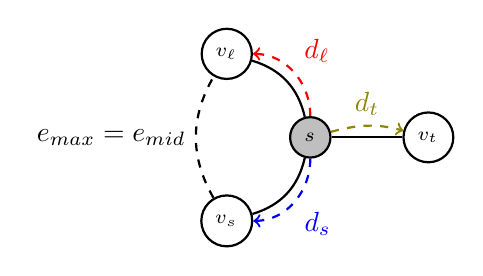
\begin{tikzpicture}[node distance={15mm}, thick, main/.style = {draw, circle}, scale=0.5] 
            \node[main, minimum size=0.5cm] (2) {$_{v_s}$ }; 
            \node[main, fill=gray!50, minimum size=0.5cm] (3) [above right of = 2] {$_{s}$ }; 
            \node[main, minimum size=0.5cm] (4) [above left of = 3] {$_{v_\ell}$ };
            \node[main, minimum size=0.5cm] (6) [right of = 3] {$_{v_t}$ };
            \draw (2) [bend left, dashed] to node[left] {$e_{max} = e_{mid}$} (4);
            \draw (2) [bend right] to node[right] {} (3);
            \draw (3) [bend right] to node[above right] {} (4);
            \draw (3) [] to node[above] {} (6);
            \path [red, thick, dashed, ->] (3) edge[out=90,in=0] node[above right] {{$d_\ell$}} (4);
            \path [blue, thick, dashed, ->] (3) edge[out=270,in=0] node[below right] {{$d_s$}} (2);
            \path [olive, thick, dashed, ->] (3) edge[out=15,in=165] node[above] {{$d_t$}} (6);
        \end{tikzpicture} 
        \hspace*{2em}
        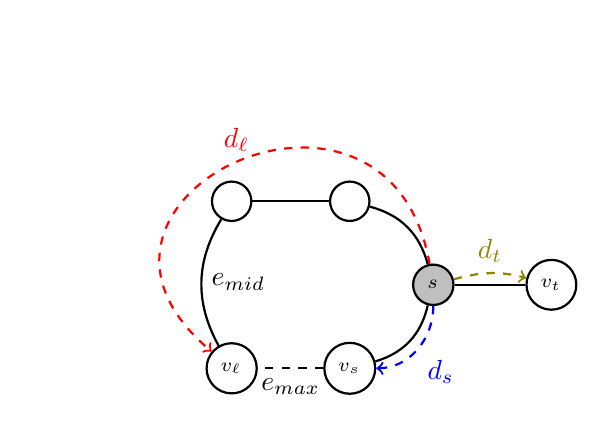
\begin{tikzpicture}[node distance={15mm}, thick, main/.style = {draw, circle}, scale=0.5] 
            \node[main, minimum size=0.5cm] (2) {$_{v_s}$ }; 
            \node[main, fill=gray!50, minimum size=0.5cm] (3) [above right of = 2] {$_{s}$ }; 
            \node[main, minimum size=0.5cm] (4) [above left of = 3] {};
            \node[main, minimum size=0.5cm] (6) [right of = 3] {$_{v_t}$ };
            \node[main, minimum size=0.5cm] (7) [left of = 2] {$_{v_\ell}$ };
            \node[main, minimum size=0.5cm] (8) [left of = 4] {};
            \draw (7) [bend left] to node[right] {$e_{mid}$} (8);
            \draw (2) [bend right] to node[right] {} (3);
            \draw (3) [bend right] to node[above right] {} (4);
            \draw (3) [] to node[above] {} (6);
            \draw (2) [dashed] to node[below] {$e_{max}$} (7);
            \draw (4) [] to node[above] {} (8);
            \path [red, thick, dashed, ->] (3) edge[looseness=2.6, bend angle=90, out=100,in=140] node[above] {{$d_\ell$}} (7);
            \path [blue, thick, dashed, ->] (3) edge[out=270,in=0] node[below right] {{$d_s$}} (2);
            \path [olive, thick, dashed, ->] (3) edge[out=15,in=165] node[above] {{$d_t$}} (6);
        \end{tikzpicture} 
        \caption[ALE at intersection]{The two possible cases when the agents start at the intersection of the tadpole graph.\linebreak Left: $e_{mid}=e_{max}$, Right: $e_{mid}\neq e_{max}$.}
    \end{center}
    \label{Case2ALE}
\end{figure}

\paragraph*{Starting at the intersection}
In this case we can use three agents to reach a competitive ratio of $2$. This is achieved by sending one agent in each direction, where only the agent seeing the shortest
edge traverses this edge at any given time. If all three agents see edges of the same length the agent that will traverse the next edge is picked at random. If two agents see
the same edge all nodes on the cycle have been visited, the third agent must be located on the tail and completes the exploration of the tail. Since only one agent moves at any
given time, the agents exploring the cycle will always stop at both sides of one of the edges with the highest length in the cycle, which will then be considered to be $e_{max}$.\\
We denote the maximum distance traversed by an agent exploring the cycle in the online strategy until all nodes have been visited as $opt_\ell$. As shown in Figure \ref{Case2ALE}, we consider two cases: 
$e_{max} = e_{mid}$ and $e_{max} \neq e_{mid}$. In the first case, we know that $d_\ell = \opt_\ell \leq L/2$. This leads to a competitive ratio of at most~$2$. 

\begin{align*}
    \small
    \opt &= 2\max(d_t, d_\ell)\\
    \onl &= d_t + d_s + d_\ell + \max(d_t, d_\ell)\\
    &\leq 4\max(d_t, d_\ell) = 2\opt\\
\end{align*}

In the second case, where $e_{max} \neq e_{mid}$, we know that $d_s + l(e_{max}) \leq opt_\ell \leq L/2 \leq d_\ell$, since $p_\ell$ must include $e_{mid}$ to be the longer path to a neighbor of $e_{max}$.
Because of this, in the online case, when all nodes have been visited, the shortest distance to $s$ is $d_s + l(e_{max})$. We also know that $d_l + d_s = L - l(e_{max}) \leq L - l(e_{mid}) \leq 2\opt_\ell$.
Because of this, we also achieve a competitive ratio of $2$ in this case.

\begin{align*}
    \small
    \opt &= 2\max(d_t, \opt_\ell)\\
    \onl &= d_t + d_s + d_\ell + \max(d_t, d_s + l(e_{max}))\\ 
    \text{Case 1: } d_s + l(e_{max}) \leq \opt_\ell \leq d_t&:\\
    \opt &= 2d_t\\
    \onl &= d_s+d_\ell+2d_t \leq 2\opt_\ell + 2d_t\\ 
    &\leq 4d_t = 2\opt\\
    \text{Case 2: } d_s + l(e_{max}) \leq d_t \leq \opt_\ell&:\\
    \opt &= 2\opt_\ell\\
    \onl &= d_s + d_\ell + 2d_t \leq 2\opt_\ell + 2d_t\\
    &\leq 4\opt_\ell = 2\opt\\
    \text{Case 3: } d_t \leq d_s + l(e_{max}) \leq \opt_\ell&:\\
    \opt &= 2\opt_\ell\\
    \onl &= 2d_s + d_\ell + l(e_{max}) + d_t \leq d_s + d_\ell + 2\opt_\ell\\
    &\leq 4\opt_\ell = 2\opt
\end{align*}

\begin{figure}[H]
    \begin{center}
        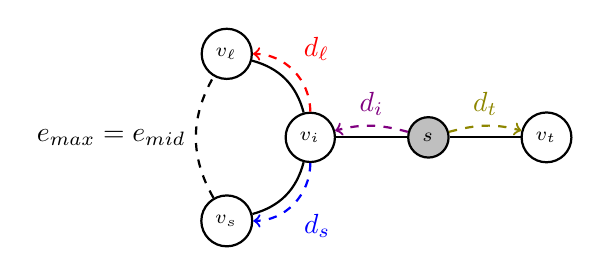
\begin{tikzpicture}[node distance={15mm}, thick, main/.style = {draw, circle}, scale=0.5] 
            \node[main, minimum size=0.5cm] (2) {$_{v_s}$ }; 
            \node[main, minimum size=0.5cm] (3) [above right of = 2] {$_{v_i}$ }; 
            \node[main, minimum size=0.5cm] (4) [above left of = 3] {$_{v_\ell}$ };
            \node[main, fill=gray!50, minimum size=0.5cm] (6) [right of = 3] {$_{s}$ };
            \node[main, minimum size=0.5cm] (7) [right of = 6] {$_{v_t}$ };
            \draw (2) [bend left, dashed] to node[left] {$e_{max} = e_{mid}$} (4);
            \draw (2) [bend right] to node[right] {} (3);
            \draw (3) [bend right] to node[above right] {} (4);
            \draw (3) [] to node[above] {} (6);
            \draw (6) [] to node[above] {} (7);
            \path [red, thick, dashed, ->] (3) edge[out=90,in=0] node[above right] {{$d_\ell$}} (4);
            \path [blue, thick, dashed, ->] (3) edge[out=270,in=0] node[below right] {{$d_s$}} (2);
            \path [olive, thick, dashed, ->] (6) edge[out=15,in=165] node[above] {{$d_t$}} (7);
            \path [violet, thick, dashed, ->] (6) edge[out=165,in=15] node[above] {{$d_i$}} (3);
        \end{tikzpicture} 
        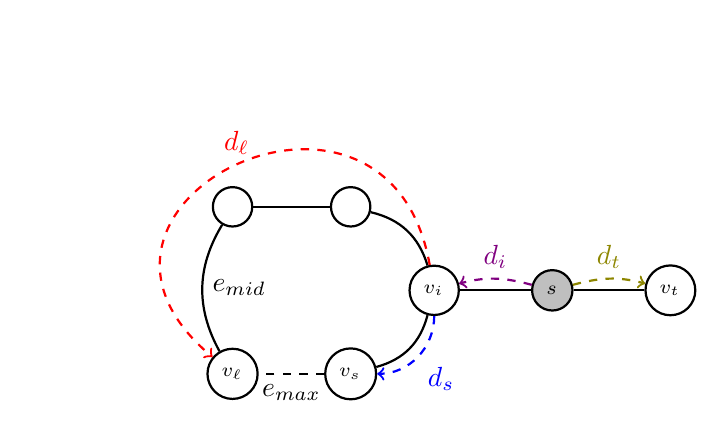
\begin{tikzpicture}[node distance={15mm}, thick, main/.style = {draw, circle}, scale=0.5] 
            \node[main, minimum size=0.5cm] (2) {$_{v_s}$ }; 
            \node[main, minimum size=0.5cm] (3) [above right of = 2] {$_{v_i}$ }; 
            \node[main, minimum size=0.5cm] (4) [above left of = 3] {};
            \node[main, fill=gray!50, minimum size=0.5cm] (6) [right of = 3] {$_{s}$ };
            \node[main, minimum size=0.5cm] (7) [left of = 2] {$_{v_\ell}$ };
            \node[main, minimum size=0.5cm] (8) [left of = 4] {};
            \node[main, minimum size=0.5cm] (9) [right of = 6] {$_{v_t}$ };
            \draw (7) [bend left] to node[right] {$e_{mid}$} (8);
            \draw (2) [bend right] to node[right] {} (3);
            \draw (3) [bend right] to node[above right] {} (4);
            \draw (3) [] to node[above] {} (6);
            \draw (2) [dashed] to node[below] {$e_{max}$} (7);
            \draw (4) [] to node[above] {} (8);
            \path [red, thick, dashed, ->] (3) edge[looseness=2.6, bend angle=90, out=100,in=140] node[above] {{$d_\ell$}} (7);
            \path [blue, thick, dashed, ->] (3) edge[out=270,in=0] node[below right] {{$d_s$}} (2);
            \path [olive, thick, dashed, ->] (6) edge[out=15,in=165] node[above] {{$d_t$}} (9);
            \path [violet, thick, dashed, ->] (6) edge[out=165,in=15] node[above] {{$d_i$}} (3);
            \draw (6) [] to node[above] {} (9);
        \end{tikzpicture}
        \caption[ALE at intersection]{The two possible cases when the agents start on the tail of the tadpole graph.\linebreak Left: $e_{mid}=e_{max}$, Right: $e_{mid}\neq e_{max}$.} 
    \end{center}
    \label{Case3ALE}
\end{figure}

\paragraph*{Starting on a node from the tail}
In this case, which is shown in Figure \ref{Case3ALE}, we use three agents to reach a competitive ratio of $2$. At the beginning of the exploration,
one agent is sent in each of the two visible directions, following the \textit{ALE} strategy, while the third agents waits at $s$. As soon as $v_i$ is found, the
third agents traverses to the intersection while the other two agents wait. From that point on, the graph is explored in all visible directions until each node has been visited.
Like in the previous case, if $e_{mid} = e_{max}$, the paths traversed by both strategies match, and we achieve a competitive ratio of $2$.

\begin{align*}
    \small
    \opt &= 2\max(d_t, d_i + d_\ell)\\
    \onl &= d_t + (d_i + d_s) + (d_i + d_\ell) + \max(d_t, d_i + d_\ell)\\
    &\leq 4\max(d_t, d_i + d_\ell) = 2\opt\\
\end{align*}

If $e_{mid} \neq e_{max}$, the relationships between the paths in the cycle from the previous cases still hold, keeping the competitive ratio at $2$.

\begin{align*}
    \small
    \opt &= 2\max(d_t, d_i + \opt_\ell)\\
    \onl &= d_t + (d_i + d_s) + (d_i + d_\ell) + \max(d_t, d_i + d_s + l(e_{max}))\\
    \text{Case 1: } d_i + d_s + l(e_{max}) \leq d_i + \opt_\ell \leq d_t&:\\
    \opt &= 2d_t\\
    \onl &= 2d_t + 2d_i + d_\ell + d_s \leq 2d_t + 2\opt_\ell + 2d_i\\
    &\leq 4d_t = 2\opt\\
    \text{Case 2: } d_i + d_s + l(e_{max}) \leq d_t \leq d_i + \opt_\ell&:\\
    \opt &= 2\opt_\ell + 2d_i\\
    \onl &= 2d_t + 2d_i + d_\ell + d_s \leq 2\opt_\ell + 4d_i + d_\ell + d_s\\
    &\leq 4\opt_\ell + 4d_i = 2\opt\\
    \text{Case 3: } d_t \leq d_i + d_s + l(e_{max}) \leq d_i + \opt_\ell&:\\
    \opt &= 2\opt_\ell + 2d_i\\
    \onl &= d_t + 3d_i + 2d_s + d_\ell + l(e_{max})\\
    &\leq 4d_i + 2d_s + l(e_{max}) + d_\ell + \opt_\ell\\
    &= 4d_i + d_s + d_\ell + 2\opt_\ell\\
    &\leq 4d_i + 4\opt_\ell = 2\opt
\end{align*}

\begin{figure}[H]
    \begin{center}
        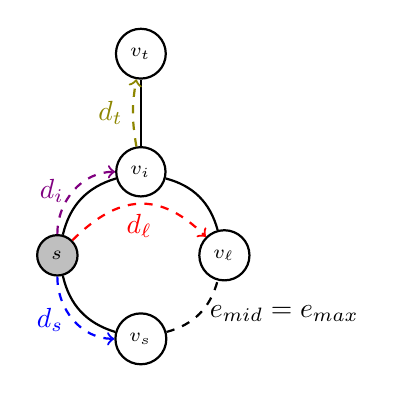
\begin{tikzpicture}[node distance={15mm}, thick, main/.style = {draw, circle}, scale=0.5] 
            \node[main, fill=gray!50, minimum size=0.5cm] (1) [] {$_{s}$ }; 
            \node[main, minimum size=0.5cm] (2) [above right of = 1] {$_{v_i}$ }; 
            \node[main, minimum size=0.5cm] (3) [below right of = 1] {$_{v_s}$ }; 
            \node[main, minimum size=0.5cm] (4) [below right of = 2] {$_{v_\ell}$ }; 
            \node[main, minimum size=0.5cm] (5) [above of = 2] {$_{v_t}$ }; 
            \draw (1) [bend left] to node[above] {} (2);
            \draw (1) [bend right] to node[above] {} (3);
            \draw (2) [bend left] to node[above] {} (4);
            \draw (3) [bend right, dashed] to node[right] {$e_{mid} = e_{max}$} (4);
            \draw (2) [] to node[above] {} (5);
            \path [red, thick, dashed, ->] (1) edge[looseness=1.25, out=45,in=135] node[below] {{$d_\ell$}} (4);
            \path [blue, thick, dashed, ->] (1) edge[out=270,in=180] node[left] {{$d_s$}} (3);
            \path [olive, thick, dashed, ->] (2) edge[out=100,in=260] node[left] {{$d_t$}} (5);
            \path [violet, thick, dashed, ->] (1) edge[out=90,in=180] node[left] {{$d_i$}} (2);
        \end{tikzpicture} 
        \hspace*{2em}
        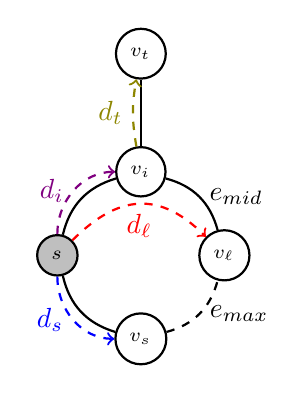
\begin{tikzpicture}[node distance={15mm}, thick, main/.style = {draw, circle}, scale=0.5] 
            \node[main, fill=gray!50, minimum size=0.5cm] (1) [] {$_{s}$ }; 
            \node[main, minimum size=0.5cm] (2) [above right of = 1] {$_{v_i}$ }; 
            \node[main, minimum size=0.5cm] (3) [below right of = 1] {$_{v_s}$ }; 
            \node[main, minimum size=0.5cm] (4) [below right of = 2] {$_{v_\ell}$ }; 
            \node[main, minimum size=0.5cm] (5) [above of = 2] {$_{v_t}$ }; 
            \draw (1) [bend left] to node[above] {} (2);
            \draw (1) [bend right] to node[above] {} (3);
            \draw (2) [bend left] to node[right] {$e_{mid}$} (4);
            \draw (3) [bend right, dashed] to node[right] {$e_{max}$} (4);
            \draw (2) [] to node[above] {} (5); 
            \path [red, thick, dashed, ->] (1) edge[looseness=1.25, out=45,in=135] node[below] {{$d_\ell$}} (4);
            \path [blue, thick, dashed, ->] (1) edge[out=270,in=180] node[left] {{$d_s$}} (3);
            \path [olive, thick, dashed, ->] (2) edge[out=100,in=260] node[left] {{$d_t$}} (5);
            \path [violet, thick, dashed, ->] (1) edge[out=90,in=180] node[left] {{$d_i$}} (2);
        \end{tikzpicture} 
    \end{center}
    \caption[ALE at intersection]{The two possible cases when the agents start on the cycle of the tadpole graph.\linebreak Left: $e_{mid}=e_{max}$, Right: $e_{mid}\neq e_{max}$.}
    \label{Case4ALE}
\end{figure}

\paragraph*{Starting on a node from the cycle}
In this case, which is shown in Figure \ref{Case4ALE}, we use four agents to reach a competitive ratio of $2$, while using three agents leads to a competitive ratio of $3$. We first show the competitive ratio of $2$
for the four agent case. After that we show why a team of three agents only achieves a competitive ratio of $3$ in this case. With a team of four agents, two agents are sent in each direction, taking
all steps in parallel, until $v_i$ is found by one of the two agent teams. At this point, the team at $v_i$ splits and the exploration continues. Note that this case cannot be distinguished from the previous case
by an online algorithm because the agents only see a node with a degree of $2$ when starting the exploration, but since using this strategy saves exactly $d_i$, it is still $2$-competitive when
starting on a node of the tail. Like in the previous cases, if $e_{mid} = e_{max}$, the paths traversed by both strategies match, and we achieve a competitive ratio of $2$.
 
\begin{align*}
    \small
    \opt &= 2\max(d_t + d_i, d_\ell)\\
    \onl &= d_t + d_i + d_s + d_\ell + \max(d_t + d_i, d_\ell)\\
    &\leq 4\max(d_t + d_i, d_\ell) = 2\opt\\
\end{align*}

If $e_{mid} \neq e_{max}$, the relationships between the paths in the cycle from the previous cases still hold, keeping the competitive ratio at $2$.

\begin{align*}
    \small
    \opt &= 2\max(d_t + d_i, \opt_\ell)\\
    \onl &= d_t + d_i + d_s + d_\ell + \max(d_t + d_i, d_s + l(e_{max}))\\
    \text{Case 1: } d_s + l(e_{max}) \leq \opt_\ell \leq d_i + d_t&:\\
    \opt &= 2d_i + 2d_t\\
    \onl &= d_s + d_\ell + d_i + 2d_t \leq 2\opt_\ell + d_i + 2d_t\\
    &\leq 3d_i + 4d_t \leq 4d_i + 4d_t = 2\opt\\
    \text{Case 2: } d_s + l(e_{max}) \leq d_i + d_t \leq \opt_\ell&:\\
    \opt &= 2\opt_\ell\\
    \onl &= d_s + d_\ell + 2d_t + d_i \leq 2\opt_\ell + 2d_t + d_i\\
    &\leq 4\opt_\ell = 2\opt\\
    \text{Case 3: } d_i + d_t \leq d_s + l(e_{max}) \leq \opt_\ell&:\\
    \opt &= 2\opt_\ell\\
    \onl &= 2d_s + l(e_{max}) + d_\ell + d_t \leq (d_s + d_\ell) + d_t + \opt_\ell\\
    &\leq (L - l(e_{max})) + 2\opt_\ell \leq 4\opt_\ell = 2\opt
\end{align*}

\begin{figure}[H]
    \begin{center}
        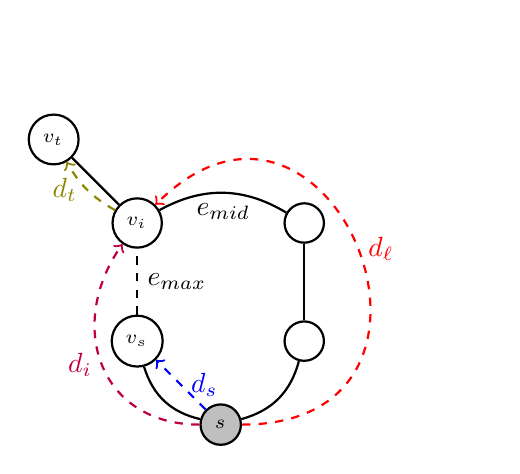
\begin{tikzpicture}[node distance={15mm}, thick, main/.style = {draw, circle}, scale=0.5] 
            \node[main, fill=gray!50, minimum size=0.5cm] (1) {$_{s}$ }; 
            \node[main, minimum size=0.5cm] (2) [above right of = 1] {}; 
            \node[main, minimum size=0.5cm] (3) [above left of = 1] {$_{v_s}$ }; 
            \node[main, minimum size=0.5cm] (4) [above of = 2] {}; 
            \node[main, minimum size=0.5cm] (5) [above of = 3] {$_{v_i}$ }; 
            \node[main, minimum size=0.5cm] (6) [above left of = 5] {$_{v_t}$ }; 
            \draw (1) [bend right] to node[above] {} (2);
            \draw (1) [bend left] to node[above] {} (3);
            \draw (2) [] to node[above] {} (4);
            \draw (3) [dashed] to node[right] {$e_{max}$} (5);
            \draw (5) [] to node[above] {} (6);
            \draw (4) [bend right] to node[below] {$e_{mid}$} (5);
            \path [red, thick, dashed, ->] (1) edge[looseness=2.7, out=0,in=45] node[right] {{$d_\ell$}} (5);
            \path [blue, thick, dashed, ->] (1) edge[out=135,in=315] node[right] {{$d_s$}} (3);
            \path [olive, thick, dashed, ->] (5) edge[out=150,in=300] node[left] {{$d_t$}} (6);
            \path [purple, thick, dashed, ->] (1) edge[looseness=1.3, out=180,in=235] node[left] {{$d_i$}} (5);
        \end{tikzpicture} 
    \end{center}
    \caption[ALE at intersection]{The special case, where $v_i$ is found on the longer path $L-d_i$ instead of the shortest path~$d_i$.}
    \label{Case5ALE}
\end{figure}

With only three agents available, the exploration strategy where the third agent waits at the start until the intersection is found only achieves a competitive ratio of $3$. Starting on a node of the cycle, there are two directions in which $v_i$ can be found. When $e_{mid} \neq e_{max}$, and $v_i$ is located on $p_\ell$,
with $L/2 < L - d_i \leq d_\ell$, the intersection can be found before the exploration of the cycle is completed, as depicted in Figure \ref{Case5ALE}. In this case the agent waiting at $s$ traverses
a distance of $L - d_i$ instead of the optimal distance of $d_i$. Since $v_i$ is located on $p_\ell$, $p_i$ must include $e_{max}$. Because of this
the exploration takes at most time $2\opt + (L - d_i) \leq 2\opt + (L - l(e_{max})) \leq 2\opt + 2\opt_\ell \leq 3\opt$, leading to a competitive upper bound of $3$ in the three agent case.
\end{proof}

\subsection{Extending the Strategies to $n$-Tadpole Graphs} \label{ntadpoles}
In this section we generalize the strategies found for tadpole graphs in \S\ref{tadpoles} onto $n$-tadpole graphs. In \S\ref{lower_bound_ntad} we show that the lower bound of $1.5$ also holds for the exploration
of $n$-tadpole graphs with any number of agents $k > 2$ in the time model. In \S\ref{ntad_two} we use the upper bound of $3$ shown by Fritsch \cite{Fritsch2021} for single-agent exploration of unicyclic graphs (graphs that contain exactly one cycle)
to construct a trivial upper bound of $12$ for two agent exploration of $n$-tadpole graphs with arbitrary $n$. This is possible, since every $n$-tadpole graph is also a unicyclic graph. In \S\ref{ntad_three} we extend the strategy using three agents on tadpole graphs to an $n+2$ agent strategy for $n$-tadpoles, reaching a competitive ratio of 
$1$ for the energy and $1.5+\frac{n}{2}$ for the time model. In \S\ref{ntad_four} the strategy using four agents on tadpole graphs is extended to a strategy using $2^{n+1}$ agents on $n$-tadpole graphs to achieve
a competitive ratio of $1.5$ for any $n$. Since any tadpole graph is also an $n$-tadpole graph, the lower bound of $1.5$ for a fixed number of two agents in the energy model
shown in Thm.\ref{TadpoleEnergyLower} still holds for $n$-tadpole graphs. The results of this section are listed in Table \ref{table:ntad}. We define $n$-tadpole graphs as follows:

\paragraph*{$n$-Tadpole Graph} An n-tadpole graph $T_n=(V,E)$ is a graph, which consists of a cycle to which
$n$ tails $T_1,...,T_n$ are attached. There can be multiple tails attached to the same cycle node. The length of the cycle will be denoted as $L_c$, the length of the tails
will be denoted as $L(T_i)$. Note that by this definition a cycle is a $0$-tadpole graph, and a tadpole graph is 
a $1$-tadpole graph. 

\begin{table}[H]
    \small
    \centering
    \begin{tabular}{|l|ll|ll|}
    \hline
               & \multicolumn{2}{c|}{Time Model}                                     & \multicolumn{2}{c|}{Energy Model}                                   \\ \hline
               & \multicolumn{1}{c|}{Lower Bound} & \multicolumn{1}{c|}{Upper Bound} & \multicolumn{1}{c|}{Lower Bound} & \multicolumn{1}{c|}{Upper Bound} \\ \hline
    $1$ Agent    & \multicolumn{1}{l|}{2 \cite{Brandt2020}}           & 3 \cite{Fritsch2021}                               & \multicolumn{1}{l|}{2 \cite{Brandt2020}}           & 3 \cite{Fritsch2021}                               \\ \hline
    $2$ Agents  & \multicolumn{1}{l|}{1.5 (Thm. \ref{nTadpoleLower})}         & 12 (Thm. \ref{nTadpoleUpperTwo})                               & \multicolumn{1}{l|}{1.5 (Thm. \ref{TadpoleEnergyLower})}            & 12 (Thm. \ref{nTadpoleUpperTwo})                               \\ \hline
    $n+2$ Agents & \multicolumn{1}{l|}{1.5 (Thm. \ref{nTadpoleLower})}         & $1.5+0.5n$ (Thm. \ref{nTadpoleUpperNplusTwo})                         & \multicolumn{1}{l|}{1}           & 1 (Thm. \ref{nTadpoleUpperNplusTwo})                                \\ \hline
    $2^{n+1}$ Agents   & \multicolumn{1}{l|}{1.5 (Thm. \ref{nTadpoleLower})}         & 1.5 (Thm. \ref{nTadpoleUpperExp})                            & \multicolumn{1}{l|}{1}           & 1 (Thm. \ref{nTadpoleUpperNplusTwo})                               \\ \hline
    \end{tabular}
    \caption{Results for multi-agent exploration of n-Tadpole Graphs.} \label{table:ntad}
\end{table}

\subsubsection{A lower bound for n-Tadpole Graphs}\label{lower_bound_ntad}

We can reuse the lower bound construction from \S\ref{lower_bound_tad} to show a lower bound of $1.5$ for the competitive ratio of any exploration of $n$-tadpole graphs,
with $k \geq 2$ Agents. We only need to show this for cases where $n\geq2$, since the lower bound of $1.5$ has already been shown for cycles by Higashikawa et al.\cite{Higashikawa2012}
and for tadpole graphs in \S\ref{lower_bound_tad}. For this, instead of one tail of length $\varepsilon$, we attach $n$ tails of length $\delta = \frac{\varepsilon}{n}$ to the starting node $s$.
Because of this the tails can still be explored in parallel to the exploration of the cycle, so the analysis from \S\ref{lower_bound_tad} still holds, since using more than
two agents for the exploration of a cycle cannot lower its exploration time.


\begin{theorem}[A lower bound for $n$-tadpole graphs]\label{nTadpoleLower}
    For any number of agents $k \geq 2$, there exists no online graph exploration algorithm with a lower competitive ratio than $1.5$ for the time model.
\end{theorem}
\vspace*{-1em}

\begin{figure}[H]
    \small
    \begin{center}
    \begin{tikzpicture}[node distance={15mm}, thick, main/.style = {draw, circle}, scale=0.5] 
        \node[main, fill=gray!50, minimum size=0.5cm] (3) [] {$_{s}$ }; 
        \node[main, minimum size=0.5cm] (2) [below left of = 3] {$_{c_3}$ }; 
        \node[main, minimum size=0.5cm] (4) [below right of = 3] {$_{c_2}$ };
        \node[main, minimum size=0.5cm] (6) [above left of = 3] {$_{t_1}$ };
        \node[main, minimum size=0.5cm] (7) [above right of = 3] {$_{t_n}$ };
        \node (8) at ($(6)!0.5!(7)$) {...};
        \draw (2) [] to node[below] {$1$} (4);
        \draw (2) [] to node[above left] {$1$} (3);
        \draw (3) [dashed] to node[above right] {$(J-3)\varepsilon$} (4);
        \draw (3) [] to node[left] {$\delta$} (6);
        \draw (3) [] to node[right] {$\delta$} (7);
        \draw (3) [] -- ($(6)!0.3!(7) - (0,0.2)$);
        \draw (3) [] -- ($(6)!0.5!(7) - (0,0.2)$);
        \draw (3) [] -- ($(6)!0.7!(7) - (0,0.2)$);
    \end{tikzpicture} 
    \hspace*{5em}
    \begin{tikzpicture}[node distance={15mm}, thick, main/.style = {draw, circle}] 
        \node[main, fill=gray!50, minimum size=0.5cm] (3) [] {$_{s}$ }; 
        \node[main, minimum size=0.5cm] (2) [below left of = 3] {$_{c_3}$ }; 
        \node[main, minimum size=0.5cm] (4) [below right of = 3] {$_{c_2}$ };
        \node[main, minimum size=0.5cm] (6) [above left of = 3] {$_{t_1}$ };
        \node[main, minimum size=0.5cm] (7) [above right of = 3] {$_{t_n}$ };
        \node (8) at ($(6)!0.5!(7)$) {...};
        \draw (2) [] to node[below] {$\varepsilon$} (4);
        \draw (2) [] to node[above left] {$1$} (3);
        \draw (3) [dashed] to node[above right] {$j\varepsilon \leq (J-3)\varepsilon$} (4);
        \draw (3) [] to node[left] {$\delta$} (6);
        \draw (3) [] to node[right] {$\delta$} (7);
        \draw (3) [] -- ($(6)!0.3!(7) - (0,0.2)$);
        \draw (3) [] -- ($(6)!0.5!(7) - (0,0.2)$);
        \draw (3) [] -- ($(6)!0.7!(7) - (0,0.2)$);
    \end{tikzpicture} 
    \end{center}
    \small\caption[Tadpole lower bound]{Any number of agents $k\geq2$ cannot explore the given graph with a competitive ratio lower than $1.5$. The dashed line is a path consisting entirely of edges with length $\varepsilon$.
    Case 1 (Left): the graph an adversary reveals if $(s, c_3)$ is not traversed after an agent traversed a distance of $(J-3)\varepsilon$ on the path between $s$ and $c_2$.
    Case 2 (Right): the graph an adversary creates when $(s,c_3)$ is traversed before an agent traverses a distance of $j\varepsilon\leq(J-3)\varepsilon$ on the path between $s$ and $c_2$.}
    \label{ntadpole-time}
\end{figure}

\begin{proof}
    The analysis stays the same as in \S\ref{lower_bound_tad}, except that instead of a single tail of length $\varepsilon$, $n$ tails of combined length $\varepsilon$ are explored.
\end{proof}

\subsubsection{n-Tadpole graphs with two Agents}\label{ntad_two}
We can show that a constant competitive ratio regardless of $n$ can be achieved with only two agents on any $n$-tadpole graph. 
For this we make use of a competitive upper bound of $3$ for single-agent exploration of unicyclic graphs shown by Fritsch \cite{Fritsch2021},
to show that using only a single agent to explore an $n$-tadpole graph yields a competitive upper bound of $12$ compared to an optimal exploration using two agents.


\begin{theorem}[Upper bound for two-agent n-tadpole graph exploration]\label{nTadpoleUpperTwo}
    Using the single-agent strategy for the exploration of unicyclic graphs, leads to a competitive upper bound of $12$ compared to
    an optimal offline strategy using two agents. This applies to the time- as well as the energy model.
\end{theorem}


\begin{proof}
    Let $e_{max}$ denote the length of the longest cycle edge in a given $n$-tadpole graph:
    \begin{enumerate}
        \item If $l(e_{max}) > L_c/2$ an optimal single-agent offline strategy traverses a distance of $\opt_1 = 2(L_c-l(e_{max}))+2\sum_{i=1}^{n}L(T_i)$
        \item If $l(e_{max}) \leq L_c/2$ an optimal single-agent offline strategy traverses a distance of $\opt_1 = L_c+2\sum_{i=1}^{n}L(T_i)$
    \end{enumerate}

    To explore an $n$-tadpole graph, the exploration path must at least include all but one edges of the cycle, as well as all edges of all tails. So any optimal exploration
    has a length of at least $(L_c - l(e_{max}))+\sum_{i=1}^{n}L(t_i)$. If we assume that this can be evenly split between two agents, we get the shortest exploration time of 
    $\opt_2 = 0.5(L_c - l(e_{max}))+0.5\sum_{i=1}^{n}L(t_i)$ for two agent exploration of an $n$-tadpole graph. We now show that this is at most $4$ times smaller than $opt_1$.

    \paragraph*{Case 1} $2(L_c-l(e_{max}))+2\sum_{i=1}^{n}L(T_i) = 4\opt_2$.
    \paragraph*{Case 2} $L_c/2 \leq L_c - l(e_{max})$, since $l(e_{max}) \leq L_c/2$.\\
    \hspace*{1em} Thus, $L_c+2\sum_{i=1}^{n}L(T_i) \leq 2(L_c - l(e_{max})) + 2\sum_{i=1}^{n}L(T_i) = 4\opt_2$.\\

    Since the single-agent online exploration strategy for unicyclic graphs takes at most time $3\opt_1$, it takes at most time $12\opt_2$.
\end{proof}

\subsubsection{n-Tadpole graphs with $n+2$ agents}\label{ntad_three}

The strategy from \S\ref{tadpole_three}, which used three agents to explore a tadpole graph, can be generalized to a strategy using $n+2$ agents to explore any $n$-tadpole graph.
The general idea is, that instead of taking at most time $4\max(d(s,v), v\in V)$, resulting in a competitive ratio of $2$ for the time model, we take at most time $(n+3)\max(d(s,v), v\in V)$,
resulting in a competitive ratio of $1.5+\frac{n}{2}$ for the time model, while maintaining a competitive ratio of $1$ in the energy model, since the longest distance traversed by any agent is
still $2\max(d(s,v), v\in V)$, matching the offline strategy. 


\begin{theorem}[Exploring $n$-tadpole graphs with $n+2$ agents]\label{nTadpoleUpperNplusTwo}
    A strategy for exploring an $n$-tadpole graph with $n+2$ agents can reach a competitive ratio of $1$ for the energy model, and
    a competitive ratio of $1.5+\frac{n}{2}$ for the time model.
\end{theorem}


\begin{proof}
    When starting the exploration, each outgoing edge of $s$ is assigned to an agent. The agents follow these edges one agent at a time, following the strategy from \S\ref{tadpole_three}.
    Whenever an intersection is found, one of the outgoing edges is assigned to the agent which found the intersection, while the other edges
    are assigned to agents without assigned edges. These agents will then traverse to the intersection while all other agents wait. After the agents reach
    the intersection, the exploration continues until all nodes have been visited by some agent and all agents return to $s$ by traversing the shortest paths.\\
    Since only one agent moves at any time, the paths traversed by the online strategy match the paths traversed in an optimal offline solution, for the same reasons
    as in \S\ref{tadpole_three}. Because of this, this strategy reaches a competitive ratio of $1$ for the energy model. While the optimal offline solution moves all agents in parallel, leading to an exploration time of $2\max(d(s,v), v\in V)$, the online strategy only
    moves the agents in parallel while backtracking, leading to a total exploration time of at most $(n+3)\max(d(s,v), v\in V)$ and a competitive ratio of $1.5+\frac{n}{2}$ 
    for the time model.
\end{proof}
\subsubsection{n-Tadpole graphs with $2^{n+1}$ agents}\label{ntad_four}

The $1.5$ competitive strategy for the exploration of tadpole graphs with four agents can be extended to a strategy using $2^{n+1}$ agents for the exploration
of $n$-tadpole graphs, which allows halving the teams of agents $n$ times.

    \begin{theorem}[Exploring $n$-tadpole graphs with $2^{n+1}$ agents]\label{nTadpoleUpperExp}
        A strategy for exploring an $n$-tadpole graph with $2^{n+1}$ agents can reach a competitive ratio of $1.5$ for the time model.
    \end{theorem}

\begin{proof} The strategy works similar to the one shown in \S\ref{tadpole_four}, but in this case, whenever an intersection with degree $j>2$ is found, the group of $k$ agents located on the intersection
    split into $j-1$ teams of size $\lfloor\frac{k}{j-1}\rfloor$ and continue the exploration in all unexplored outgoing directions. Since the initial team size
    is $2^{n+1}$, we never run out of agents when finding an intersection, while exploring an $n$-tadpole~graph.\\
We already know that any agent $a$ traversing some distance $d_a$, can wait at most $d_a$ time steps, before some other
agent reaches a node where the next traversed edge would increase its traversed distance to a value larger than $d_a$, or 
all other agents have reached their destinations. Because of this, the last visited node $v$ is visited after at most time $2d(s,v)$ has passed, 
leading to an exploration time of at most $3\max(d(s,v), v\in V)$ and a competitive ratio of $1.5$.
\end{proof}
